\section{Attitude Determination \& Control} \label{sec:adcs}
The ADCS is generally assumed here to include all subsystems necessary for precise pointing and slewing, except for micro-propulsion.
\subsection{Kinematics}
Given the quaternion vector expressed in the body frame relative to the inertial frame
\begin{equation}
\mathbf{q}\triangleq 
    \begin{bmatrix}
    \eta \\
    \boldsymbol{\epsilon}
    \end{bmatrix}
\end{equation}
where $\boldsymbol{\epsilon}$ is defined as
\begin{equation}
\boldsymbol{\epsilon}\triangleq 
    \begin{bmatrix}
    \epsilon_x \\
    \epsilon_y \\
    \epsilon_z
    \end{bmatrix}
\end{equation}
The kinematic differential equations may be written in compact form as
\begin{equation}
\dot{\mathbf{q}}=\frac{1}{2}
    \begin{bmatrix}
    -\boldsymbol{\epsilon}^T \\
    \eta\mathbf{I}_{3\times 3}+\mathbf{S}\left ( \boldsymbol{\epsilon} \right)
    \end{bmatrix}\boldsymbol{\omega}_{ib}^b
\end{equation}
\noindent where $\boldsymbol{\omega}_{ib}^b$ is the angular velocity of the body relative to an inertial frame. $\mathbf{S}(\boldsymbol{\epsilon})$ denotes a skew-symmetric matrix operator, given by
\begin{equation}
\mathbf{S}(\boldsymbol{\epsilon})=-\mathbf{S}(\boldsymbol{\epsilon})^{T}=\boldsymbol{\epsilon}^{\times}\triangleq
    \begin{bmatrix}
        0 && -\epsilon_z && \epsilon_y \\
        \epsilon_z && 0 && -\epsilon_x \\
        -\epsilon_y && \epsilon_x && 0 
    \end{bmatrix}
\end{equation}
\subsection{Dynamic Model}
The dynamical model for a rigid body actuated by means of external moments and subject to external disturbance moments is given by Euler’s momentum equation
\begin{equation}
    \mathbf{J}_b\dot{\boldsymbol{\omega}}^{b}_{ib}=\mathbf{S}\left (\mathbf{J}_b\boldsymbol{\omega}^b_{ib}\right )\boldsymbol{\omega}^b_{ib}+\boldsymbol{\tau}^b_a+\boldsymbol{\tau}^b_d
\end{equation}
where $\boldsymbol{\omega}^b_{ib}$ is the angular velocity of the body relative to an inertial frame, $\mathbf{J}_b$ is the body inertia matrix, $\boldsymbol{\tau}^b_a$ is the control input and $\boldsymbol{\tau}^b_d$ disturbance moments.

A mathematical model may also be expressed for an internally actuated
vehicle. The vehicle consists of an assumed rigid structure, with electronic
devices, sensors, etc., and for example four reaction wheels which are spinning about a fixed axis of inertial symmetry, such that the total moment of inertia may be assumed constant in the
body frame. Such a mechanical device, consisting of a rigid body combined with several
spinning rotors or wheels, is commonly referred to as a gyrostat. The expression for total angular momentum and axial momentum of the wheels in body frame $\mathcal{F}_b$ may be written as
\begin{subequations}
\begin{equation}
    \mathbf{h}^b=\mathbf{J}_b\boldsymbol{\omega}^b_{ib}+\mathbf{A}\mathbf{I}_w\boldsymbol{\omega}_w
\end{equation}
\begin{equation}
    \mathbf{h}_a=\mathbf{J}_b\mathbf{A}^T\boldsymbol{\omega}^b_{ib}+\mathbf{I}_w\boldsymbol{\omega}_w
\end{equation}
\end{subequations}
where $\mathbf{A} \in \mathbb{R}^{3 \times m}$ is a matrix of wheel axis body coordinates, $\mathbf{I}_w \in \mathbb{R}^{m \times m}$ a diagonal matrix of wheel inertias, $\boldsymbol{\omega}_w \in \mathbb{R}^m$ a vector of wheel velocities.
Writing in coordinate form in $\mathcal{F}_b$, we obtain 
\begin{equation}
    \dot{\mathbf{h}}^b+\mathbf{S}\left ( \boldsymbol{\omega}^b_{ib}\right ) \mathbf{h}^b+\mathbf{S}\left (\mathbf{c}^b\right)\dot{\mathbf{v}}^b=\sum{\tau}^b 
\end{equation}
\noindent where $\boldsymbol{\tau}^b_d$ are sum of torques expressed in body coordinates. Assuming that the origo coincides with the center of mass such that $\mathbf{c}^b\equiv 0$, then we obtain
\begin{subequations}
    \begin{equation}
    \dot{\mathbf{h}}^b=\mathbf{S}\left ( \mathbf{h}^b \right ) \bar{\mathbf{J}}^{-1}\left(\mathbf{h}^b-\mathbf{A}\mathbf{h}^a \right)-\boldsymbol{\tau}^b_a+\boldsymbol{\tau}^b_d
    \end{equation}
    \begin{equation}
    \dot{\mathbf{h}}_a=\boldsymbol{\tau}_a
    \end{equation}
\end{subequations}
\noindent where $\mathbf{A}$ is the reaction wheel torque distribution matrix and $\bar{\mathbf{J}} \in \mathbb{R}^{3 \times 3}$ is an inertia-like matrix defined as
\begin{equation}
     \bar{\mathbf{J}} \triangleq \mathbf{J}+\mathbf{A}\mathbf{I}_w\mathbf{A}^T
\end{equation}
Thus the dynamical model for an internally actuated satellite may be expressed as
\begin{subequations}
\begin{equation}
      \bar{\mathbf{J}}\dot{\boldsymbol{\omega}}^{b}_{ib}=\mathbf{S}\left (\bar{\mathbf{J}}\boldsymbol{\omega}^b_{ib}\right )\boldsymbol{\omega}^b_{ib}+\mathbf{S}\left (\mathbf{A}\mathbf{I}_w\boldsymbol{\omega}_w\right )\boldsymbol{\omega}^b_{ib}-\mathbf{A}\boldsymbol{\tau}^b_a+\boldsymbol{\tau}^b_e
    \end{equation}
    \begin{equation}
      \mathbf{I}_w\dot{\boldsymbol{\omega}}_w= \boldsymbol{\tau}_a-\mathbf{I}_w\mathbf{A}\dot{\boldsymbol{\omega}}^b_{ib}
      \end{equation}
\end{subequations}
The inertia matrix for \hypso may explicitly be written as
\begin{equation}
    \bar{\mathbf{J}} = \begin{bmatrix}
			0.077451 & -0.000517 & 0.00024 \\
-0.000517 & 0.106727 & -0.00015 \\
0.00024 & -0.00015 & 0.038937 \\
    \end{bmatrix}
		\end{equation}
\subsection{External Forces and Moments}
External forces and torques affect the satellite while orbiting Earth, both environmental and actuator-generated.

The gravity gradient torque in coordinate vectors expressed in the body system is given as
\begin{equation}
    \boldsymbol{\tau}_g=3\omega_o^2(z_{o3}^b)^{\times}\bar{\mathbf{J}}z_{o3}^b
\end{equation}
\noindent where $\omega_o^2=\frac{\mu}{R_c^3}$ ($R_c^3$ and $\mu$ are distance between the mass centers of two bodies and gravitational constant of the primary celestial body, $\mathbf{I}$ is the inertia dyadic and the nadir pointing vector in body coordinates is
\begin{equation}
    z_{o3}^b=\mathbf{R}_o^b\begin{bmatrix}
    0 \\
    0 \\
    1 
    \end{bmatrix}
\end{equation}
The aerodynamical torque on the satellite results from particles in the atmosphere colliding
with a non-symmetric cross section. The effects are significant at lower altitudes in LEO. In the
worst-case this torque is given by
\begin{equation}
    \boldsymbol{\tau}_{ad}=F_{ad}(c_{pa}-c_{g})\begin{bmatrix}
    0 \\
    1 \\
    0 
    \end{bmatrix}
\end{equation}
\noindent where $F_{ad}=0.5\rho C_d AV^2$ and $\rho$ is the atmospheric density, $C_d$ is the drag coefficient, $A$ is the surface area, $V$ is the spacecraft velocity, $c_{pa}$ is the aerodynamic center of pressure and $c_g$ is the center of gravity.
A controlled magnetic moment may be created by generating a torque given by
\begin{equation}
    \boldsymbol{\tau}_{m}=\mathbf{m}\times \mathbf{B}(t)
\end{equation}
\noindent where $\mathbf{m}$ is the generated magnetic moment and $\mathbf{B}(t)$ is the local magnetic field.

Solar radiation pressure may be expressed as 
\begin{equation}
    \boldsymbol{\tau}_{sp}=F_{sp}(c_{sp}-c_{g})\begin{bmatrix}
    0 \\
    1 \\
    0 
    \end{bmatrix}
\end{equation}
\noindent where $\frac{F_s}{c}A_s(1+q)\cos i$, $F_s$ is the solar constant $1.367\hspace{2pt} W/m^2$, $c$ is the speed of light, $A_s$ is the surface area, $q$ is the reflectance factor and $i$ is the angle of incidence of the Sun and $c_{sp}$ is the center of solar pressure.

The total torque due to a reaction wheel assembly is given by
\begin{equation}
    \boldsymbol{\tau}^b_{a}=\mathbf{A}\boldsymbol{\tau}_a
\end{equation}
\noindent where $\boldsymbol{\tau}_a$ is a vector of wheel torques and $\mathbf{A}$ is given by
\begin{equation}
\mathbf{A}=
    \begin{bmatrix}
        1 && 0 && 0 && \cos(54.7^{\circ}) \\
        0 && 1 && 0 && \cos(54.7^{\circ}) \\
        0 && 0 && 1 && \cos(54.7^{\circ}) 
    \end{bmatrix}
\end{equation}

\subsection{Slew Maneuver}
Based on \cite{Ack16,Dic05}, the key requirements for the HSI are chosen to be:
\begin{enumerate}
\item GSD $<$ 100 m/pixel
\item Spectral resolution of 5 nm
\end{enumerate}

In order to make the HSI payload compact (approximately 2.5 U, and
less than 600 g), several tradeoffs have been accepted. In particular
the design leads to a violation of the 100 meter/pixel GSD in the
longitudinal direction when looking Nadir. This is due to two factors:

\begin{itemize}

\item The optical resolution on the ground in the
  longitudinal direction is 500 m.

\item The satellite speed is about 7634 m/s, which leads to each pixel
  being acquired while traveling a distance of about 192.97 m with a
  frame rate of 39.56 fps (frames per second).
	
\end{itemize}

While an improvement in optical resolution requires a smaller slit
width, an improvement in the frame rate requires either a larger slit
width, or a larger and more sensitive image sensor. A more sensitive
image sensor is currently not easily available without increasing the
size and weight of the optics. However, another solution to this
problem is enabled by the assumption that the length of the ground
track is small compared to the satellite track.
\begin{figure}[htbp]
  \begin{center}
    \subfigure[Slewing motion required to point the camera towards a
    70 km longitudinal ground track while the satellite is moving in a
    414 km in-orbit track.]{\label{fig:con4-1a}\includegraphics[width=60mm,angle=0]{figs/concept4-1-2.png}}
    \subfigure[Overlapping pixels aquired by the HSI along the track, achieving $GSD <39$ m/pixel as a requirement.]{\label{fig:con4-1b}\includegraphics[width=60mm,angle=0]{figs/concept4-2-2.png}}
    \caption{\sml slewing motion and the constraints.}
    \label{fig:con4}
\end{center}
\end{figure}
As illustrated in Figure \ref{fig:con4} there are two
effects that are achieved by a slewing motion of the satellite:
\begin{enumerate}

\item The HSI is slowly scanning the 70 km ground track (assumed to be relatively stationary) over a period
  of time while the satellite moves 413.7 km in orbit. At an altitude of
  500 km, this means that initially the attitude of the satellite will
  be approximately $\theta=20^{\circ}$ deg relative to Nadir pointing, while
  at the end of the track the attitude will be approximately $\theta=-20^{\circ}$
  relative to Nadir. With a satellite moving at $v_{\text{sat}}=7634$ m/s
  speed, the attitude needs to change approximately $\Delta \theta=40^{\circ}$ during $\approx$ 57.6 s,
  i.e. at a rate close to $\omega_{y}\approx 0.7028^{\circ}$/s about the y-axis and appying torque to the x-face. The effect of this is that the first two
  pixels are acquired over $39$ m instead of 192.7 m with exposure time of $\Delta t = 25.4$ ms, contributing
  significantly to better GSD overall becoming $\leq 39$ m during the pass. Equation \ref{eq:spatial} becomes,
\begin{equation}
\Delta x = \delta x + (v_{\text{sat}}-\omega_{y} \cdot r) \Delta t \label{eq:spatial2}
\end{equation}
hence the spatial resolution of first frame, after \sml has slewed during $\Delta t = 25.4$ ms, becomes $\Delta x=559.5 $ m instead of $\Delta x=692.7 $ m for a Nadir-looking satellite. $r$ or $h/\cos(\theta)$ is taken here to be the range from the spacecraft to the ground.

\item Since the spatial resolution is $\Delta x \approx 559.5$ m and each pixel is acquired
  over $\leq 39$ m, there will be approximately 6 partially overlapping pixels that can be
  used in a deconvolution filter in order to enhance the image
  resolution. 

\end{enumerate}
Passes are illustrated in Figure \ref{fig:slewingops} showing that overlapping pixels are achieved through slewing. Two actuation segments are necessary as shown in Figure \ref{fig:slewingops2} and Figure \ref{fig:slewingops3} shows the dynamics of cross-track pointing and slewing.
\begin{figure*}[htbp]
  \centering
    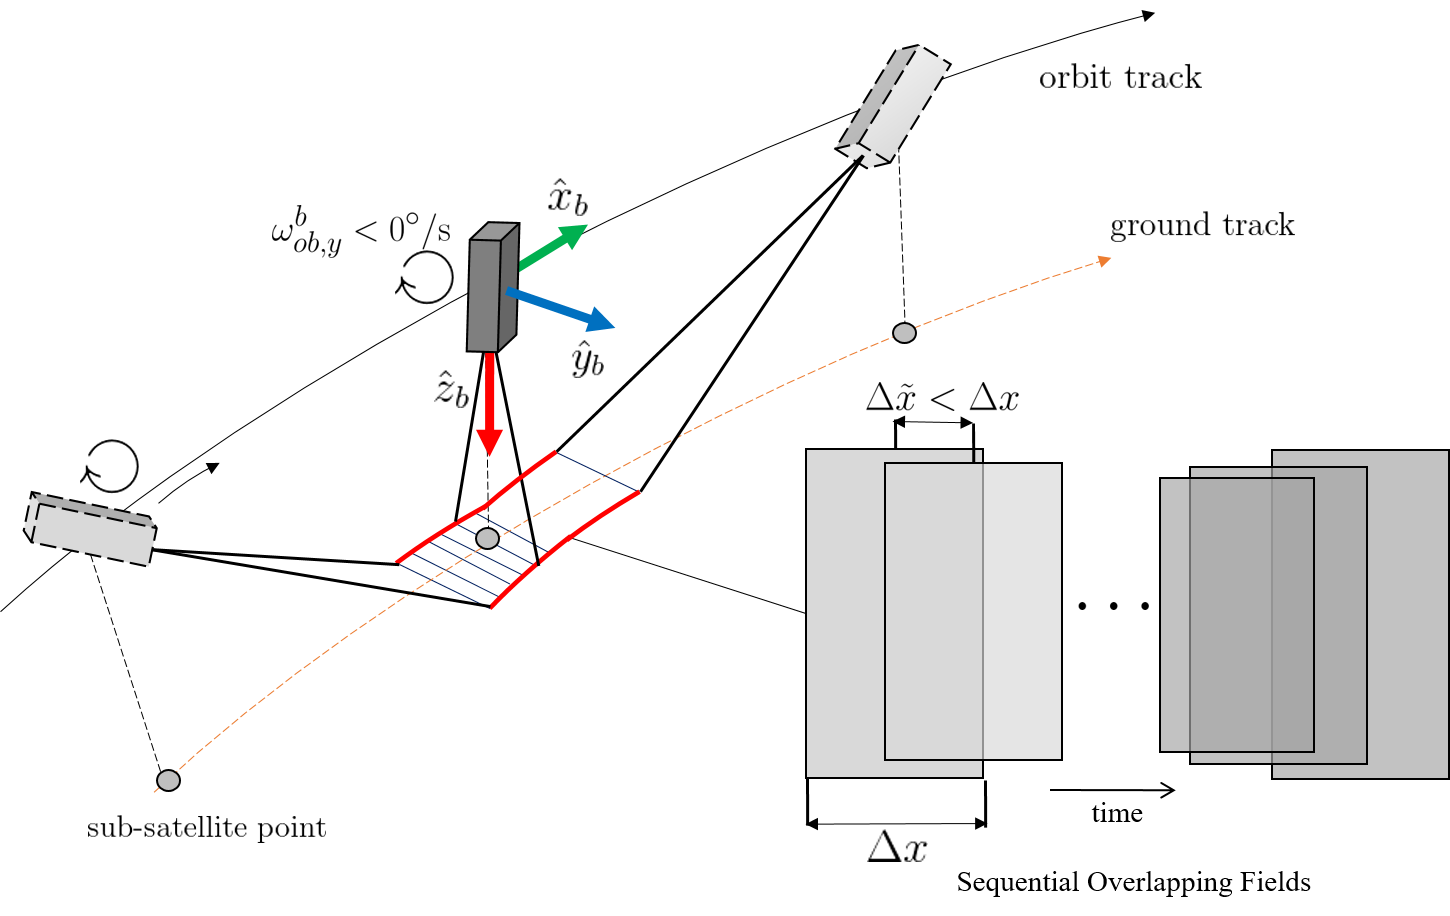
\includegraphics[width=120mm,angle=0]{figs/slew_operations.png}
    \caption{\hypso slews above a target area and achieves overlapping pixels. It has three observational passes, where two of them requires \hypso to point cross-track while slewing.}
    \label{fig:slewingops}
\end{figure*}
\begin{figure*}[htbp]
  \centering
    \includegraphics[width=90mm,angle=0]{figs/slew_operations2.png}
    \caption{\hypso slews in one plane (about y-axis), showing that two actuations are necessary. Momentum is finally dumped by magnetorquers.}
    \label{fig:slewingops2}
\end{figure*}
\begin{figure}[htbp]
  \centering
    \includegraphics[width=80mm,angle=0]{figs/slew_operations3.png}
    \caption{\hypso points cross-track to target (actively) while slewing along a line on the ground. This has limitations due to pointing accuracy and substantial movement, since references to controller are fixed roll angle and angular velocity about the y-axis of the body.}
    \label{fig:slewingops3}
\end{figure}

The target also moves during the HSI observation time slot due to Earth's rotation and needs to be accommodated for in terms of $(x,y,z)_{\text{ECEF}}$ coordinates. This inevitably creates small geometric distortions in addition to the issues coming from pointing precision of satellite\footnote{Usually $\theta_{\text{error}}\approx 0.1 ^{\circ} (2\sigma)$ is assumed for a 6U CubeSat with all necessary ADCS (Attitude Determination and Control System) components}. %Need to establish precision error and error in m (ground)
\begin{figure}[htbp]
  \centering
      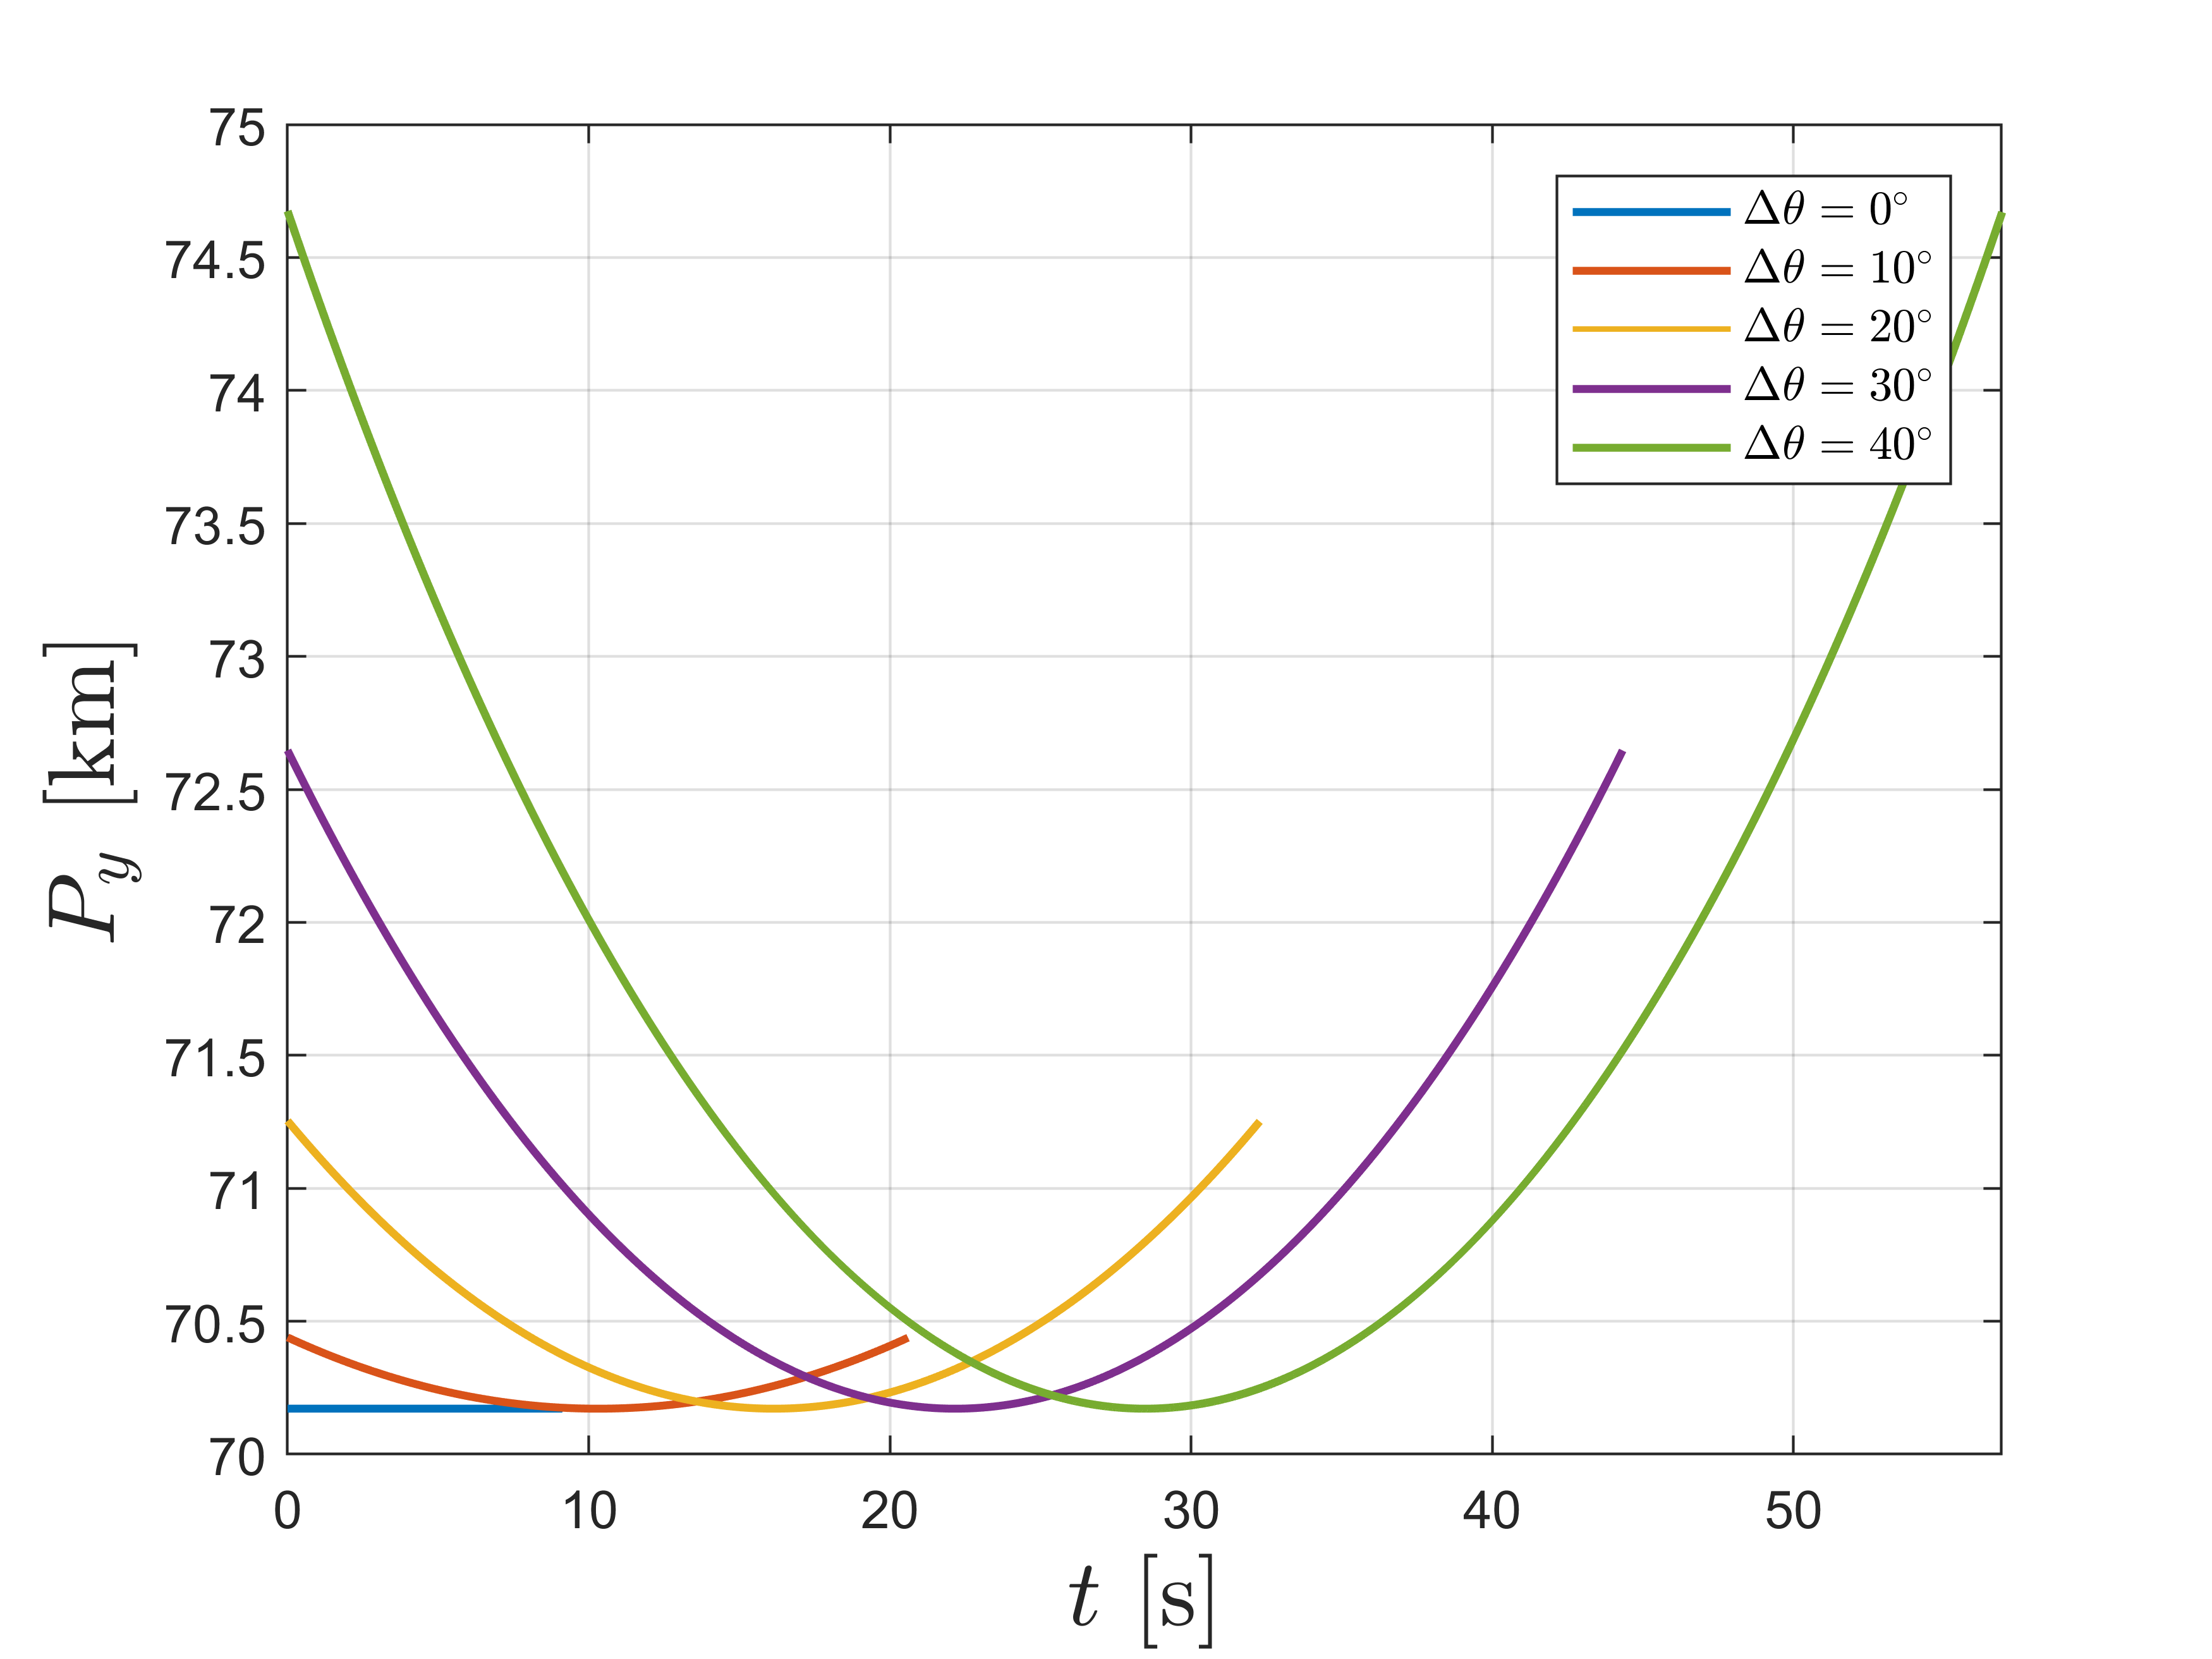
\includegraphics[width=0.4\textwidth]{figs/swath_time.png}
  \caption{Swath Width versus viewing angle. Blue: $\gamma$ =0$^{\circ}$ and $\dot{\gamma}$ =0$^{\circ}$/s, Red: $\gamma$ =10$^{\circ}$ and $\dot{\gamma}$ =0.6761$^{\circ}$/s, Orange: $\gamma$ =20$^{\circ}$ and $\dot{\gamma}$ =0.7391$^{\circ}$/s, Purple: $\gamma$ =30$^{\circ}$ and $\dot{\gamma}$ =0.7277$^{\circ}$/s}
	\label{fig:spatial_time}
\end{figure}
\begin{figure}[htbp]
  \centering
      \includegraphics[width=0.4\textwidth]{figs/optical_resolution_time.png}
  \caption{Optical resolution versus viewing angle. Blue: $\theta$ =0$^{\circ}$ and $\omega_{y}\approx 0^{\circ}$/s, Red: $\theta$ =10$^{\circ}$ and $\omega_{y}\approx 0.6197^{\circ}/s$, Orange: $\theta$ =20$^{\circ}$ and $\omega_{y}\approx 0.7028^{\circ}/s$, Purple: $\theta$ =30$^{\circ}$ and $\omega_{y}\approx 0.7065^{\circ}/s$}
	\label{fig:spatial_time}
\end{figure}
\begin{figure}[htbp]
  \centering
      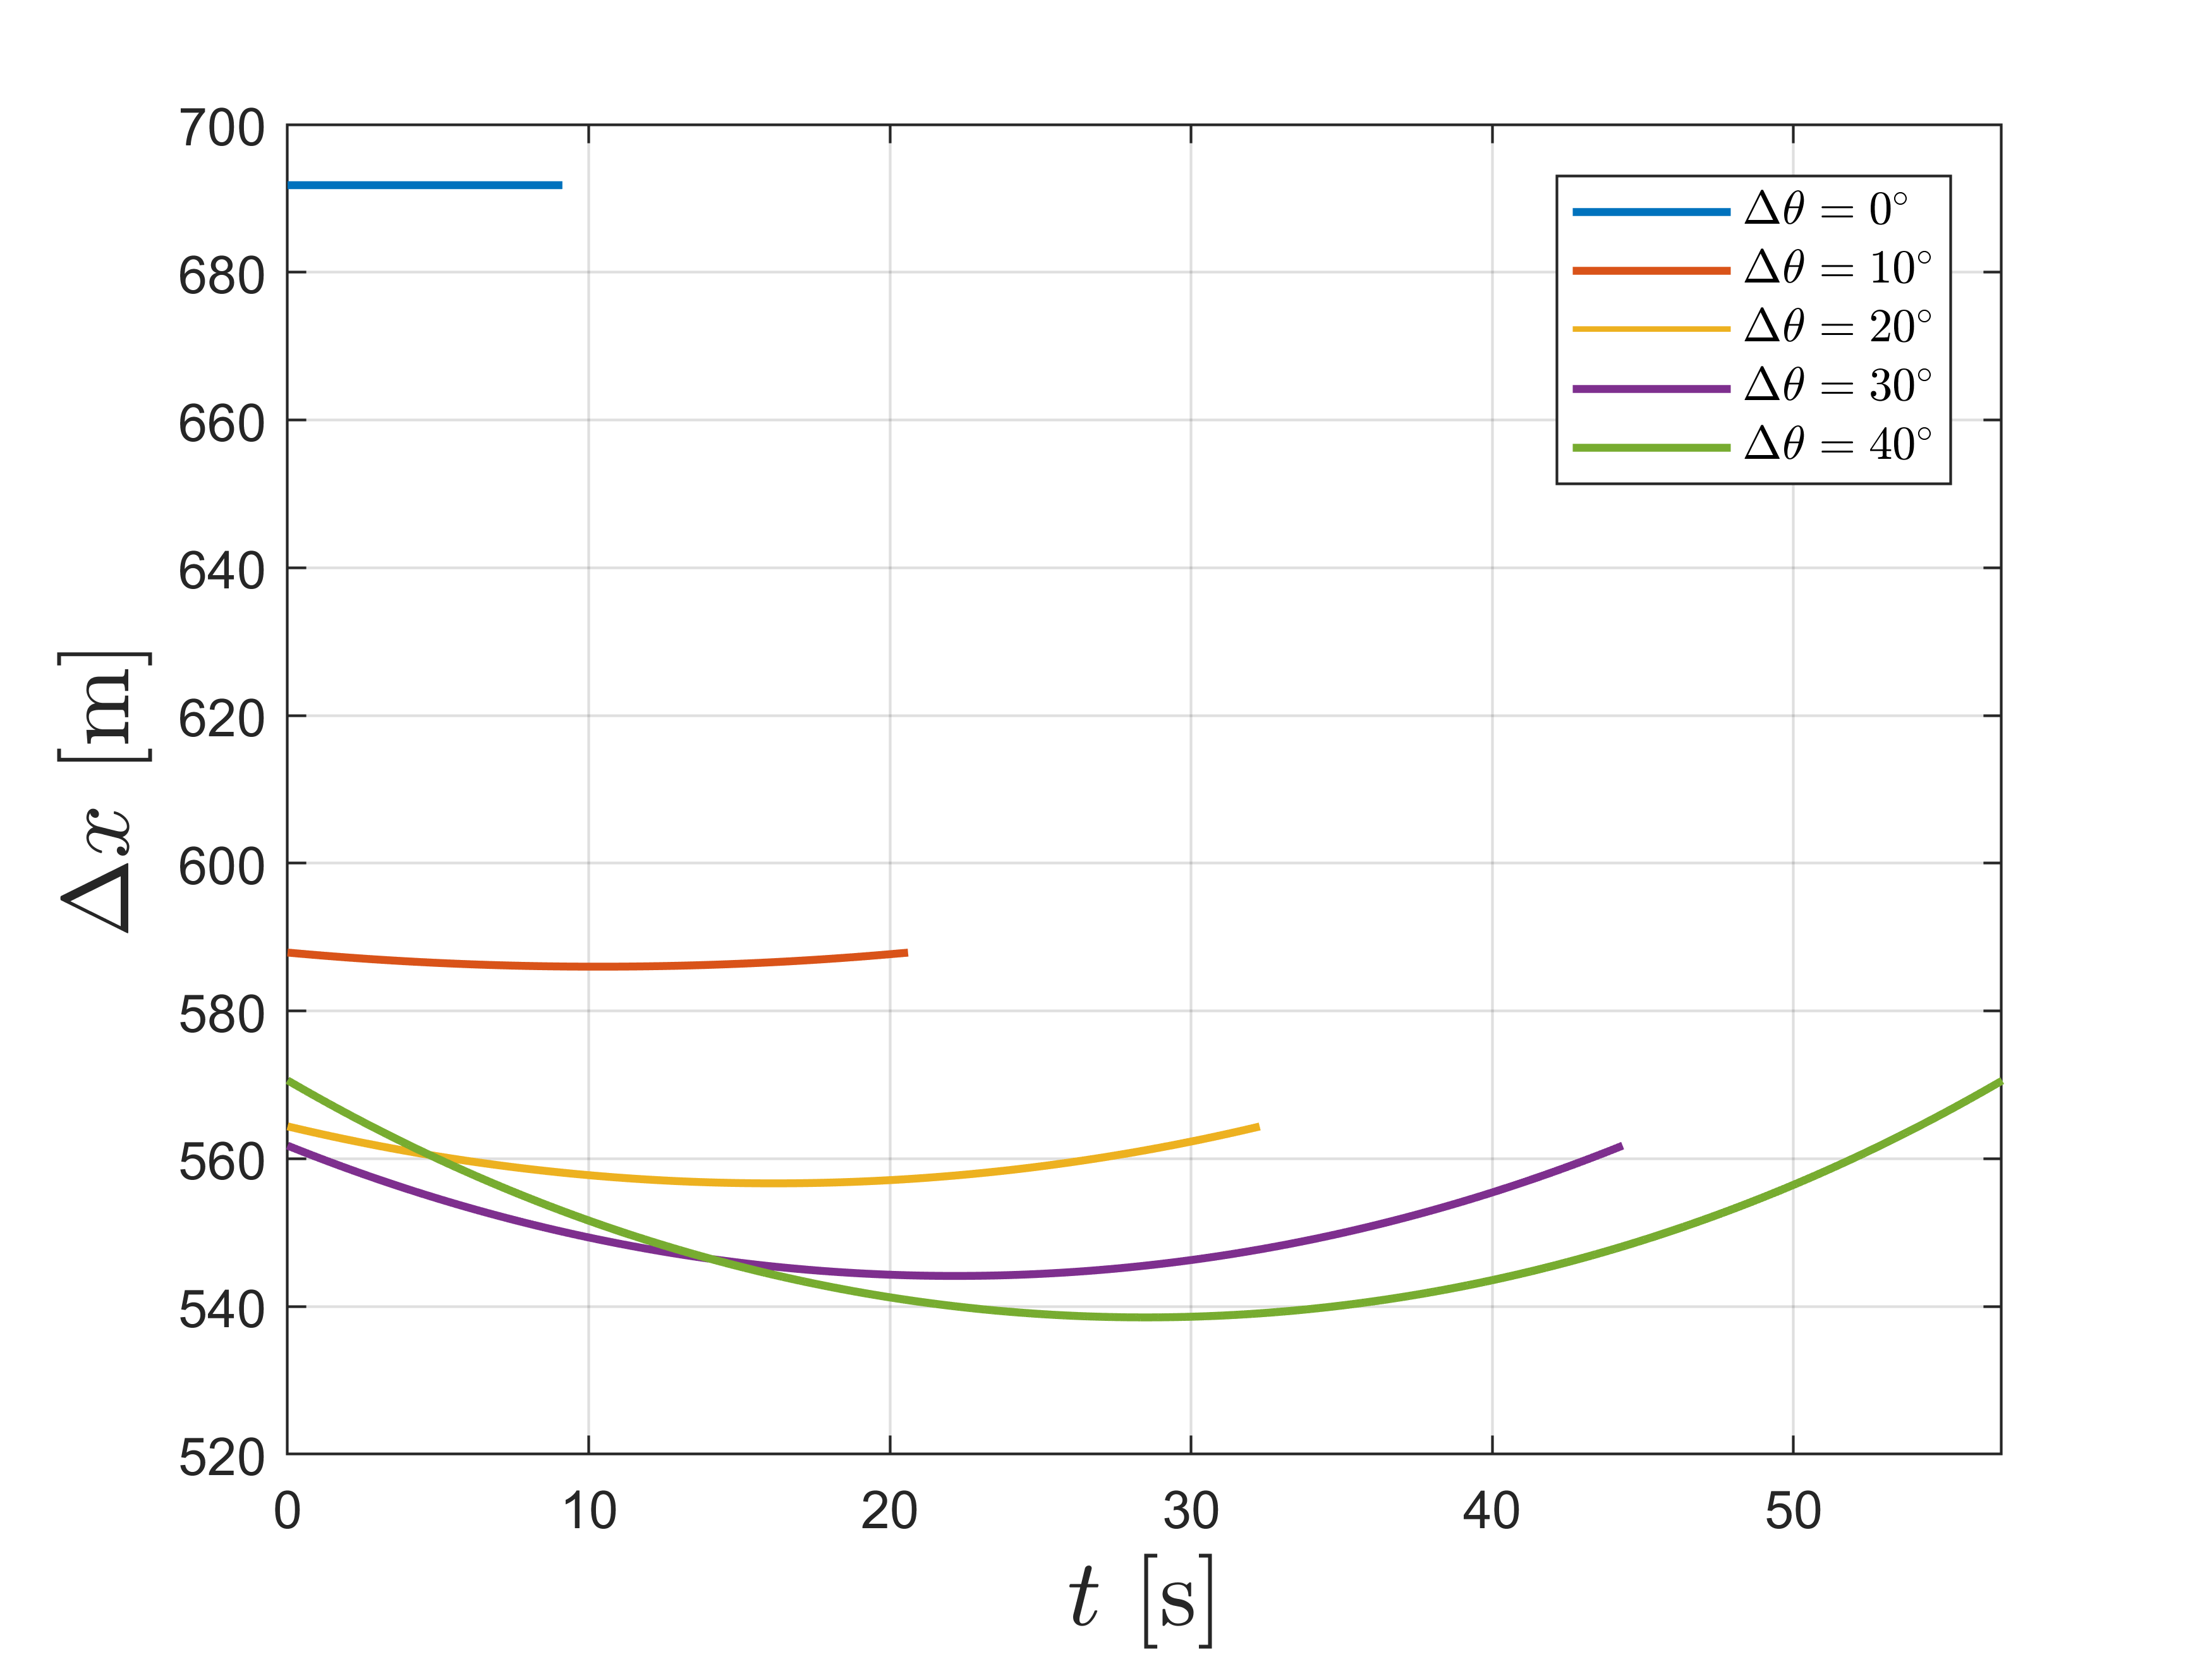
\includegraphics[width=0.4\textwidth]{figs/spatial_time.png}
  \caption{Spatial resolution versus viewing angle for $\Delta t$ =0.0254 s. Blue: $\theta$ =0$^{\circ}$ and $\omega_{y}\approx 0^{\circ}$/s, Red: $\theta$ =10$^{\circ}$ and $\omega_{y}\approx 0.6197^{\circ}/s$, Orange: $\theta$ =20$^{\circ}$ and $\omega_{y}\approx 0.7028^{\circ}/s$, Purple: $\theta$ =30$^{\circ}$ and $\omega_{y}\approx 0.7065^{\circ}/s$}
	\label{fig:spatial_time}
\end{figure}
\begin{figure}[htbp]
  \centering
      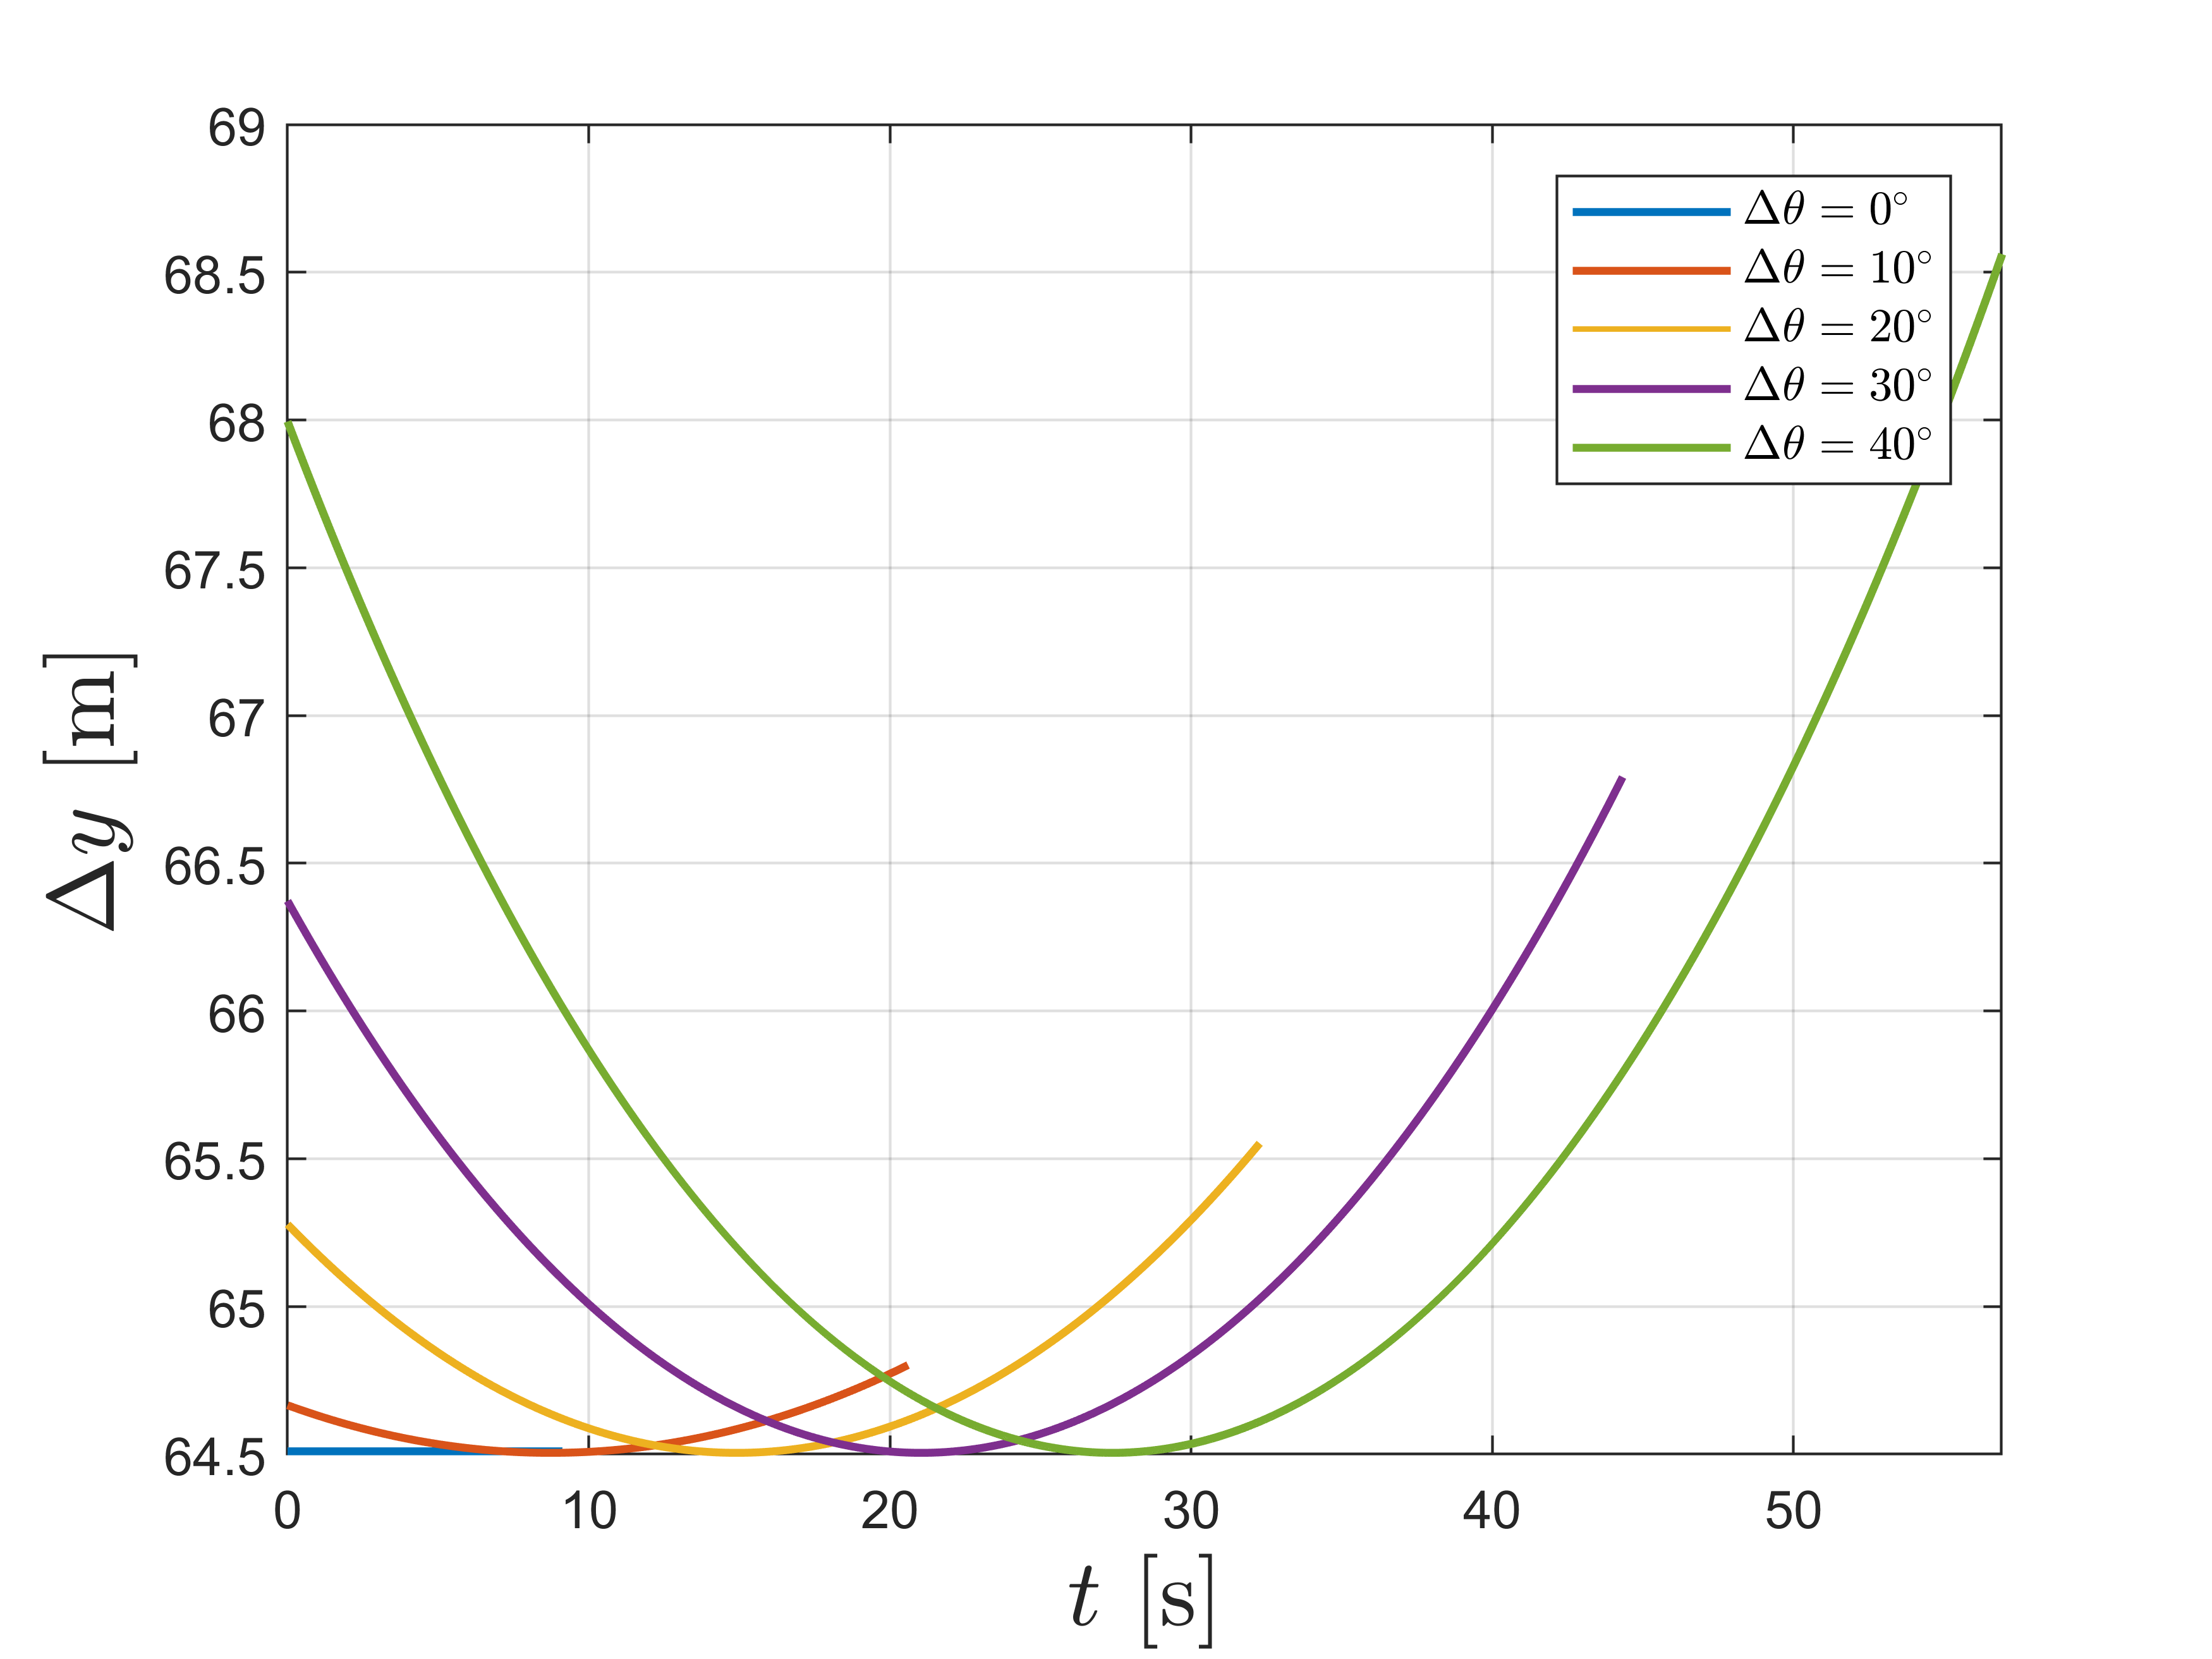
\includegraphics[width=0.4\textwidth]{figs/spatial_time_cross.png}
  \caption{Cross-track spatial resolution versus viewing angle. Blue: $\theta$ =0$^{\circ}$ and $\omega_{y}\approx 0^{\circ}$/s, Red: $\theta$ =10$^{\circ}$ and $\omega_{y}\approx 0.6197^{\circ}/s$, Orange: $\theta$ =20$^{\circ}$ and $\omega_{y}\approx 0.7028^{\circ}/s$, Purple: $\theta$ =30$^{\circ}$ and $\omega_{y}\approx 0.7065^{\circ}/s$}
	\label{fig:spatial_time}
\end{figure}
\begin{figure}[htbp]
  \centering
      \includegraphics[width=0.4\textwidth]{figs/GSD.png}
  \caption{Ground Sampling Distance vs. Time for $\Delta t$ =0.0254 s, $\theta$ =20$^{\circ}$ and $\omega_{y}\approx 0.7028^{\circ}/s$.}
	\label{fig:GSD}
\end{figure}
\begin{figure}[htbp]
  \centering
      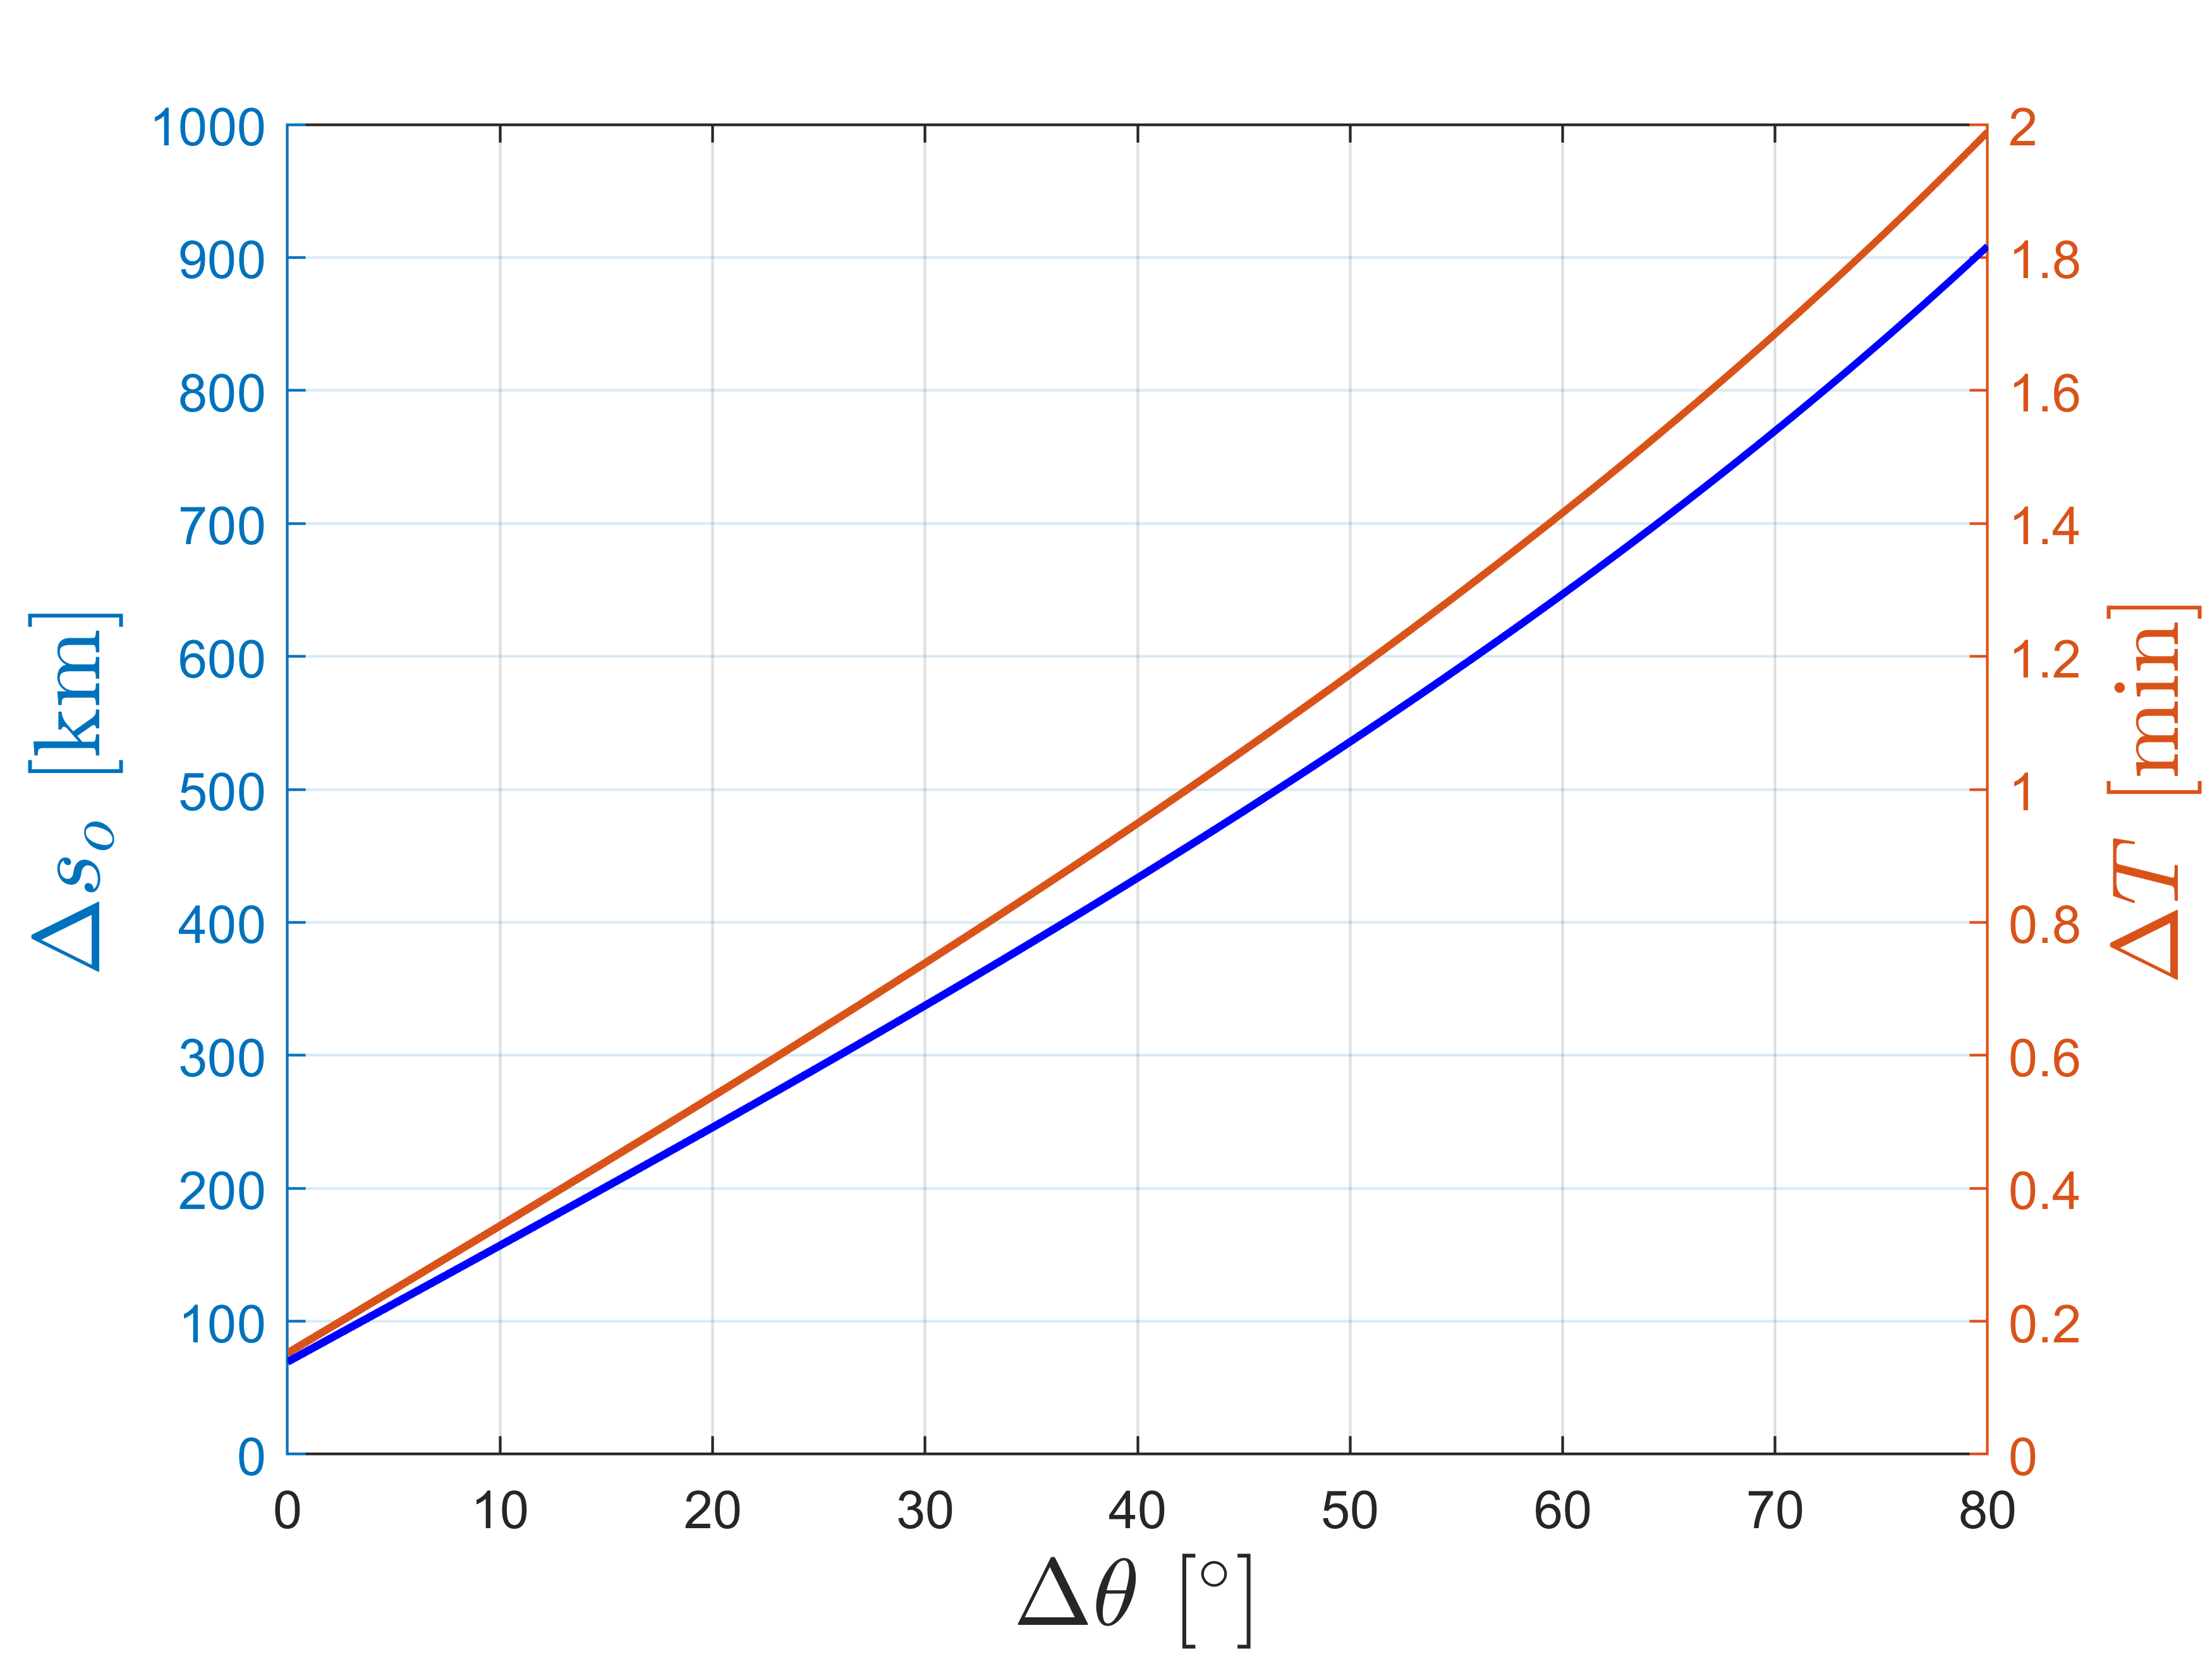
\includegraphics[width=0.4\textwidth]{figs/track_time.png}
  \caption{In-orbit track distance (km) vs. observation time}
	\label{fig:track_time}
\end{figure}
\begin{figure}[htbp]
  \centering
      \includegraphics[width=0.4\textwidth]{figs/precision_error1.png}
  \caption{Ground error during sampling for different pointing precision errors. Blue: $\delta \theta$ =0.01$^{\circ}$, Red: $\delta \theta$ =0.012$^{\circ}$, Orange: $\delta \theta$ =0.014$^{\circ}$, Purple: $\delta \theta$ =0.016$^{\circ}$, Green: $\delta \theta$ =0.018$^{\circ}$.}
	\label{fig:precision_error1}
\end{figure}
ADCS requirements are shown in \ref{tab:ADCS_requirement}
\begin{table}[htbp]
	\centering
			\caption{Slew Maneuver Conditions}
		\begin{tabular}{|l|l|}
			\hline
			\textbf{Performance}	&			\textbf{Definition} 			\\ 
			\hline
			Target area (in-track $\times$ cross-track) & 70 km $\times$ 70 km \\
			Altitude (baseline) & 500 km \\
			Exposure time & 25.4 ms \\
			Solar zenith angle & $<75^{\circ}$ \\
			In-track view angle (start; wrt. Nadir) & $+20^{\circ}$ \\
			In-track view angle (end; wrt. Nadir) & $-20^{\circ}$ \\
			In-orbit track distance & 413.7 km \\
			Time window for observation & 57.6 s \\
			GSD & $<39$ m \\
			Slew rate & $0.7028^{\circ}$/s \\
			Raw SNR per frame @ 500 nm & $\approx$ 198.73 \\
			Overlapping pixels (in-track) & 6 \\
			Total SNR per frame @ 500 nm & 485.78 (raw SNR $\times \sqrt{\text{frames}})$\\
			\hline
			\textbf{ADCS}	&			\textbf{Definition} 			\\ 
			\hline
			Orbit knowledge (GPS) & $<7$ m \\
			Pointing knowledge (S/C) & $0.01^{\circ} \hspace{3pt} (2\sigma)$ \\
			Pointing accuracy (S/C) & $0.1^{\circ} \hspace{3pt} (2\sigma)$ \\
			Drift error (gyroscope) & $1^{\circ}$/hr \\
			S/C stability & $0.06^{\circ}$/hr \\
			Controller stability & $0.01^{\circ}$ \\
			Settling time & 60 s \\
			Mapping error & $<$100 m \\
			Clock error & $<$1 ms \\
			\hline
		\end{tabular}
	  \label{tab:ADCS_requirement}
\end{table}
\subsection{Reaction Wheel Design} \label{sec:reactionwheeldesign}
The mission requirement of slewing at least $\omega_{y}=0.7028^{\circ}/s$ is equivalent to $\Delta \theta= 40^{\circ}$ during 57.6 s image acquisition. This will achieve in-track Ground Sampling Distance of $<39 \hspace{2pt} m$ of a $70 \hspace{2pt} km$ long target area at $500 \hspace{2pt} km$ altitude. This enables overlapping fields of view to be fused through super-resolution or deconvolution algorithms to enable even higher image resolution than the camera's optical resolution. Given the requirement and constraints, we assume that $1^{\circ}/s$ is the worst case along one axis with respect to Nadir. 

The total angular rotation $\theta$ produced by a reaction wheel within a given time $t_f$ gives the maximum angular momentum for the satellite 
\begin{equation}
    h_{\text{max}} = \frac{2I_{\text{max}}\Delta \theta}{t_f}
\end{equation}
where $I_{\text{max}}$ is the greatest inertia of the satellite: for a $6 \hspace{2pt} kg$ 3U CubeSat this is equivalent to $I_{xx}=I_{yy}=0.05 \hspace{2pt} kgm^2$ and for a $6.7 \hspace{2pt} kg$ 6U CubeSat this is $I_{yy}=0.0975 \hspace{2pt} kgm^2$. By selecting a motor with a maximum wheel speed of (average case) $\omega_{\text{max}}=3700$ rpm, inertia for one wheel can be found as
\begin{equation}
    I_{\text{total}} = \frac{ h_{\text{max}}}{\omega_{\text{max}}}
\end{equation}
Knowing that for worst case mass and size of reaction wheel when modeled as a disk then
\begin{equation}
    I_{\text{total}} = I_{\text{disk}} = \frac{m_{\text{disk}}r^2_{\text{disk}}}{2}
\end{equation}
where $m_{\text{disk}}=\rho\pi r^2_{\text{disk}}h_{\text{disk}}$, $\rho$ is the density of iron $7.35\cdot10^{3} \hspace{2pt} kg/m^3$, $r_{\text{disk}}$ is the radius of the disk and $h_{\text{disk}}$ is its height. We also assume that the height of the disk is equal to
\begin{equation}
    h_{\text{disk}} = \frac{r_{\text{disk}}}{2}
\end{equation}
Let's consider a 6U structure with mass $m = 6.7 \hspace{2pt} kg$ with $I_{\text{max}}=0.0975 \hspace{2pt} kgm^2$. Rearranging the equations above we get that, for a slew rate requirement of $1^{\circ}/s$ during 57.6 seconds, that we would require aluminum material reaction wheel of radius $r_{\text{disk}}\geq 25.68 \hspace{2pt} mm$, height $h_{\text{disk}} \geq 12.84 \hspace{2pt} mm$ and mass $m_{\text{disk}} \geq 0.0719 \hspace{2pt} kg$. Figs. \ref{fig:RW_mass}, \ref{fig:RW_radius} and \ref{fig:RW_torque} show the systems sizing for different slew rates when mapping the same target area.
\begin{figure}[htbp]
  \centering
    \includegraphics[width=80mm,angle=0]{figs/reactionwheel_mass.png}
    \caption{Reaction Wheel Design Mass vs. Slew Rate}
    \label{fig:RW_mass}
\end{figure}
\begin{figure}[htbp]
  \centering
    \includegraphics[width=80mm,angle=0]{figs/reactionwheel_radius.png}
    \caption{Reaction Wheel Design Radius vs. Slew Rate}
    \label{fig:RW_radius}
\end{figure}
\begin{figure}[htbp]
  \centering
    \includegraphics[width=80mm,angle=0]{figs/reactionwheel_torque.png}
    \caption{Reaction Wheel Design Torque vs. Slew Rate}
    \label{fig:RW_torque}
\end{figure}
\section{Modeling \& Simulation} \label{sec:simulations}
\begin{figure}[htbp]
  \centering
    \includegraphics[width=80mm, angle=0]{figs/Cubemodel.png}
    \caption{Representation of the 6U CubeSat model with COM indicated at the geometric center (0,0,0)}
    \label{fig:cubesat_model}
\end{figure}
\subsection{Simulations} \label{sec:simulations}
The state vector may be defined as
\begin{equation}
   \mathbf{x} = \begin{bmatrix}
   \theta & \phi & \psi & \omega^{b}_{ob,x} & \omega^{b}_{ob,y} & \omega^{b}_{ob,z} \\
   \end{bmatrix}^{T}
\end{equation}
The simulations are performed on a 6U CubeSat with tetrahedral configured reaction wheels without disturbance model. Actuators are assumed to be NanoAvionics' Reaction Wheels with specifications in \footnote{\url{https://n-avionics.com/subsystems/cubesat-reaction-wheels-control-system-satbus-4rw/}}. Sampling is chosen to be at 4 Hz.

\subsubsection{Motor Controller}
The motor wheel speed is controlled by the reference wheel speed found by the spacecraft controller (outer loop). Block diagram is shown in Fig. \ref{fig:RW_dynamics}. The inner loop is at least sampled at the same or higher than the outer loop (4 Hz). A PI controller is chosen for the motor wheel regulation with following transfer function
\begin{equation}
G(s)=K_{p,\text{motor}}+\frac{K_{i,\text{motor}}}{s}
\end{equation}
with the gains set to $K_{p,\text{motor}}=0.017$ and $K_{i,\text{motor}}=0.055$. Saturations are $V_{\text{max}}=5 \hspace{5pt} V$, $i_{a,\text{max}}=0.6 \hspace{5pt} A$, $\omega_{w,{\text{max}}}=6500 \hspace{5pt} RPM$ and $\tau_{a,{\text{max}}}=3.2 \hspace{5pt} mNm$. For instance, if motor speed is sampled at half of the time of the outer loop, then we have the speed tracking as shown in Figure \ref{fig:motor_speed_track}.
\begin{figure*}[htbp]
  \centering
    \includegraphics[width=120mm, angle=0]{figs/RW_dynamics.png}
    \caption{Block diagram for the motor wheel dynamics}
    \label{fig:RW_dynamics}
\end{figure*}
\begin{figure}[htbp]
        \centering
        \includegraphics[width=80mm, angle=0]{figs/motor_speed_track.png}
		    \caption{Motor Speed Regulator Output}
		\label{fig:motor_speed_track}
		\end{figure}
\subsubsection{PD Controller}
Simulations are performed with external perturbations on a reference angular velocity-tracking satellite, with initial conditions set to
\begin{equation}
   \mathbf{x} = 
	\begin{bmatrix}
   0 & 0 & 0 & 1\times10^{-6} & 1\times10^{-6} & 1\times10^{-6} \\
   \end{bmatrix}^{T}
\end{equation}
and reference state is
\begin{equation}
   \boldsymbol{\omega}^{b}_{ob,d} = 
	\begin{bmatrix}
   0 & 0.7028^{\circ}/s & 0 \\
   \end{bmatrix}^{T}
\end{equation}
The PD controller for the slew maneuver is chosen as
\begin{equation}
    \boldsymbol{\tau}_a^b =  k_p \cdot \boldsymbol{\omega}^{b}_{ob,e} + k_d \cdot \dot{\boldsymbol{\omega}}^{b}_{ob,e} 
		= k_p \cdot \begin{bmatrix}
    \omega^{b}_{ob,x} \\
   \omega^{b}_{ob,y} \\
   \omega^{b}_{ob,z}
   \end{bmatrix}_{e} + k_d \cdot \begin{bmatrix}
    \dot{\omega}^{b}_{ob,x} \\
   \dot{\omega}^{b}_{ob,y} \\
   \dot{\omega}^{b}_{ob,z}
   \end{bmatrix}_{e}
\end{equation}
where selected gains are $k_p=4\cdot10^{-2}$ and $k_d=1\cdot10^{-3}$. 
Figurs \ref{fig:euler_plot}-\ref{fig:control_input_plot_power} show the results for the PD controller with selected gains. After 150 s, then \hypso reorients itself to Nadir with reference
\begin{equation}
   \mathbf{x}_d = 
	\begin{bmatrix}
   0 & 0 & 0 & 0 & 0 & 0 \\
   \end{bmatrix}^{T}
\end{equation}
\noindent and PD controller
\begin{equation}
    \boldsymbol{\tau}_a^b =  k_p \cdot \boldsymbol{\epsilon}_{e} + k_d \cdot \boldsymbol{\omega}^{b}_{ob,e} 
\end{equation}
\noindent with gains $k_p=1.5\times10^{-4}$ and $k_d=2\times10^{-3}$.
    \begin{figure}[htbp]
        \centering
        \includegraphics[width=80mm, angle=0]{figs/euler_plot.png}
				\caption{Attitude}
				\label{fig:euler_plot}
    \end{figure}%
	
    \begin{figure}[htbp]
        \centering
        \includegraphics[width=80mm, angle=0]{figs/ang_vel_plot.png}
				\caption{Angular Velocity}
				\label{fig:ang_vel_plot}
    \end{figure}
		
		\begin{figure}[htbp]
        \centering
        \includegraphics[width=80mm, angle=0]{figs/motor_speed_plot.png}
				\caption{Motor speed}
				\label{fig:motor_speed_plot}
    \end{figure}
				\begin{figure}[htbp]
        \centering
        \includegraphics[width=80mm, angle=0]{figs/control_input_plot.png}
				\caption{Torque}
				\label{fig:control_input_plot}
    \end{figure}
		
			\begin{figure}[htbp]
        \centering
        \includegraphics[width=80mm, angle=0]{figs/control_input_current_plot.png}
				\caption{Current Control signal}
				\label{fig:control_input_plot_voltage}
    \end{figure}
				\begin{figure}[htbp]
        \centering
        \includegraphics[width=80mm, angle=0]{figs/control_input_power_plot.png}
				\caption{Power Consumption}
				\label{fig:control_input_plot_power}
    \end{figure}
\subsection{Errors}
There are several orientation errors to consider while imaging a target on ground or pointing actively towards a Ground Station. These include S/C position errors (in-track, cross-track, radial), sensing axis orientation errors (elevation, azimuth), target altitude error, clock errors. Other errors may be mechanical such as e.g. thermal expansions, micro-vibrations and jittering. Pointing errors relate to the imprecision in attitude control and angular motion, while mapping errors concern about the angular motion during the exposure as well as attitude and orbit knowledge (hence most relevant for the slewing maneuver proposed for the HSI mission). The need to understand the sources of errors comes from trade-off analysis between cost vs. performance (size of S/C, how many \# of reaction wheels, need for star-tracker, processing power for controllers etc.). Mapping and pointing errors due to fixed sources as a function of S/C viewing angle are shown in Figs. \ref{fig:mappingerror} and \ref{fig:pointingerror}
\begin{figure}[htbp]
  \centering
    \includegraphics[width=80mm,angle=0]{figs/Mapping_error.png}
    \caption{Mapping errors due to S/C subsystem sources.}
    \label{fig:mappingerror}
\end{figure}
\begin{figure}[htbp]
  \centering
    \includegraphics[width=80mm,angle=0]{figs/Pointing_error.png}
    \caption{Pointing errors due to S/C subsystem sources.}
    \label{fig:pointingerror}
\end{figure}